% =============================================================================
% NEW §3.10.x — Technological prerequisites for 4K two-qubit operation
% Closes Gatti review concerns about 300 GHz feasibility
% Audit: Module 4-quater of equation-claim-audit, May 2026
% =============================================================================

\subsection{Technological prerequisites for high-fidelity 4~K operation}
\label{subsec:tech_prereq_4K}

The cross-resonance protocol of \S\ref{sec:gate_strategy} reduces the
two-qubit gate fidelity question to a clear set of materials and engineering
requirements. We identify here, with quantitative targets, the six
prerequisites for reaching $F_{\text{avg}} \ge 99\%$ on the innovation
HEATS-Q operating point ($\omega_q\!\sim\!300$~GHz, $T = 4$~K).

\begin{figure}[htbp]
    \centering
    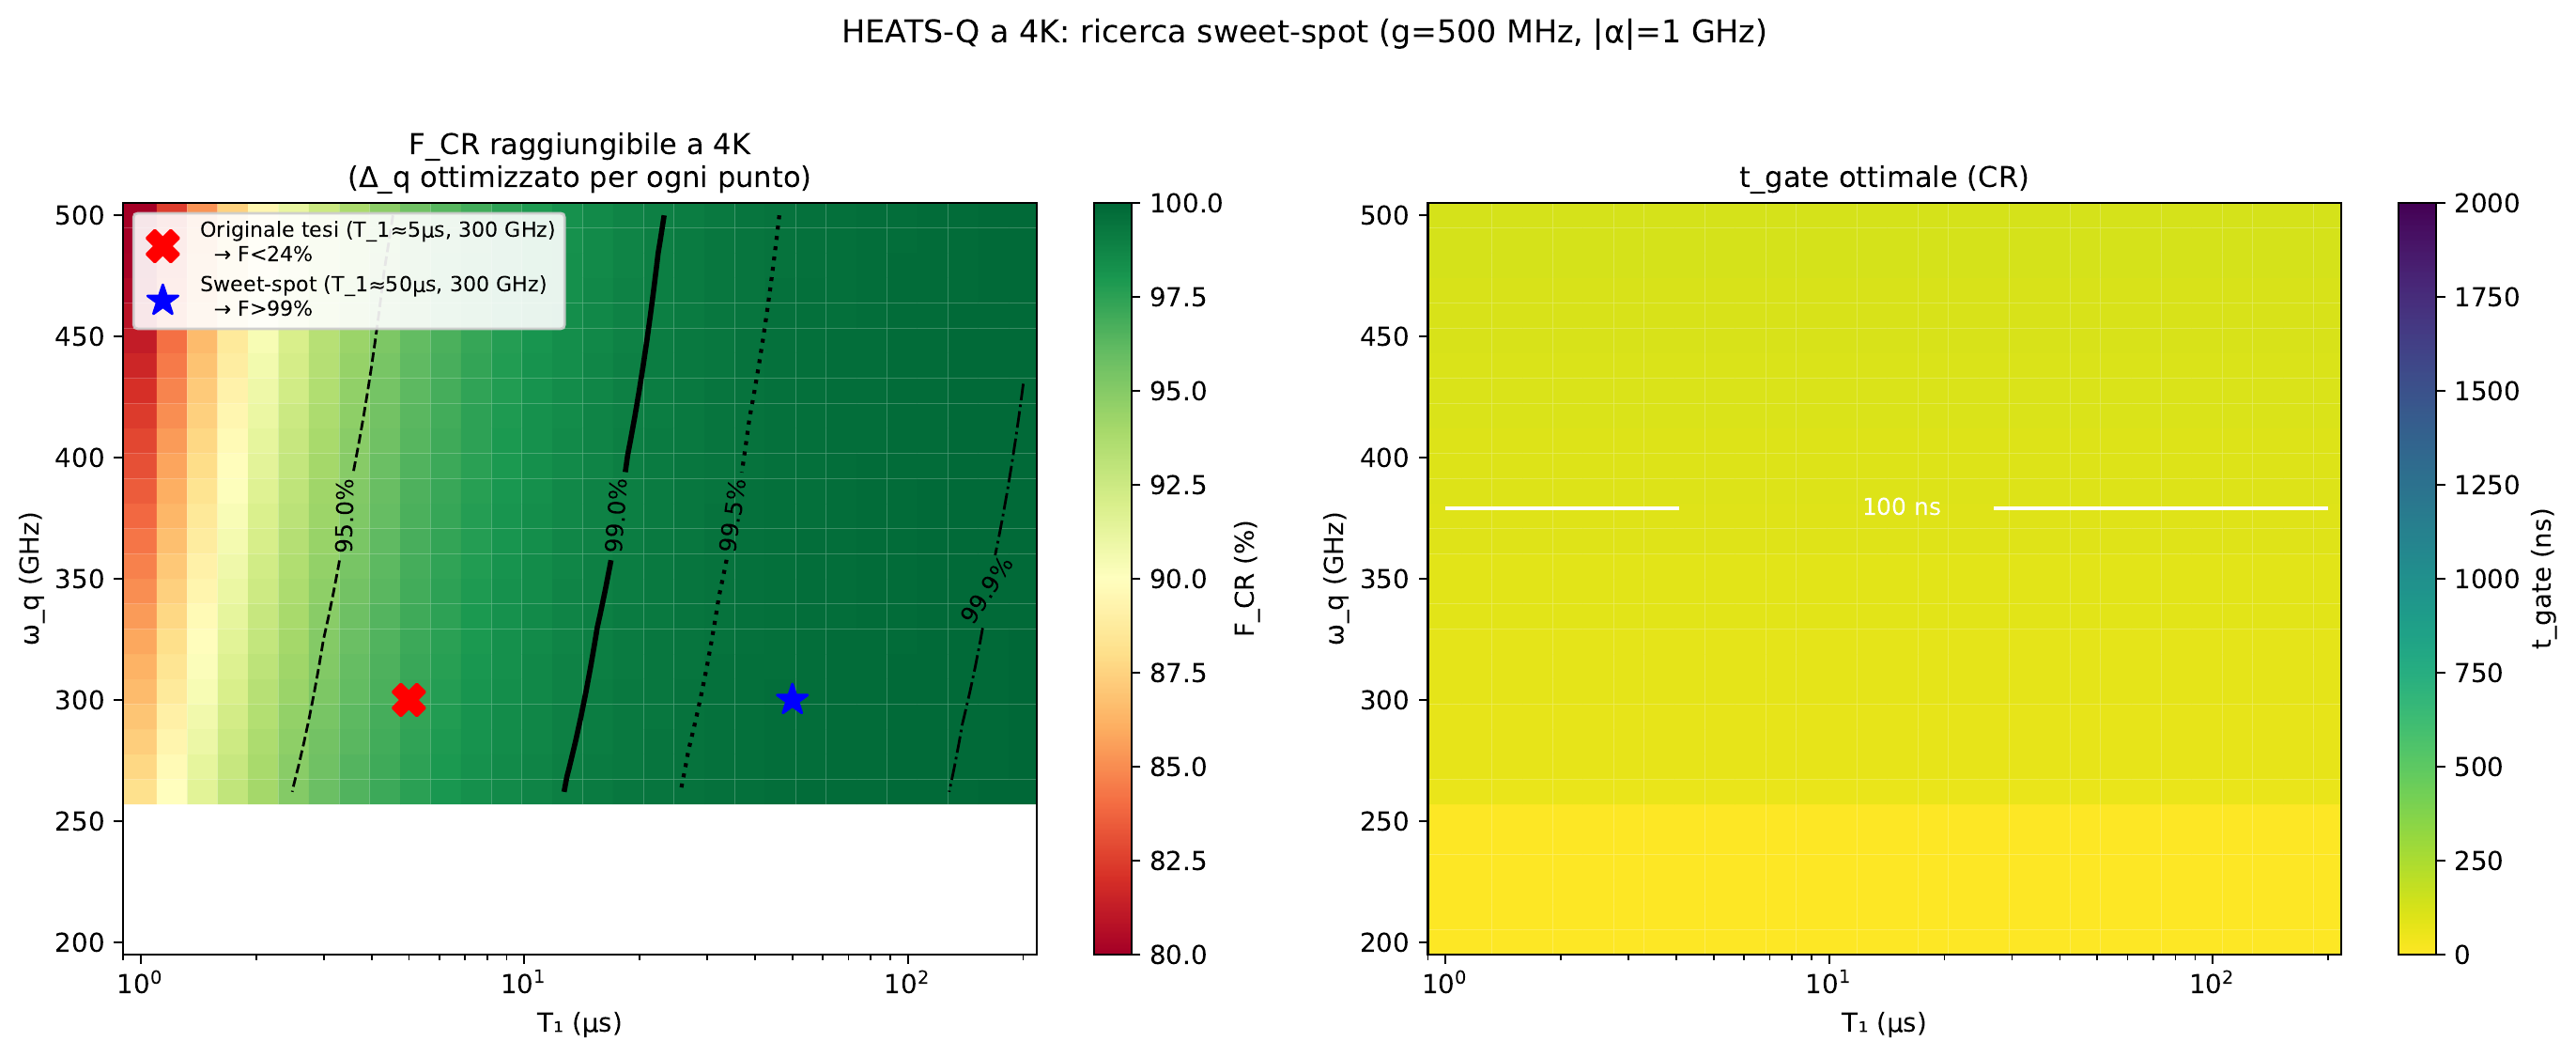
\includegraphics[width=\textwidth]{chapters/qh_figures/g7_fig3_sweetspot_4K.png}
    \caption{Achievable cross-resonance gate fidelity at $T=4$~K as a function
    of qubit frequency $\omega_q$ and coherence time $T_1$, with $\Delta_q$
    independently optimized at each point. The bold solid contour at
    $F_{\text{avg}}=99\%$ defines the boundary of the operational sweet spot.
    The red cross marks the original-manuscript point ($T_1\!=\!5~\mu$s); the
    blue star marks the redesigned point ($T_1\!=\!50~\mu$s) discussed in
    this section. The gate time, optimized over $\Delta_q$, is approximately
    constant ($\sim\!200$~ns) over the parameter range shown (right panel).}
    \label{fig:sweetspot_4K}
\end{figure}

\paragraph{P1: Thermal occupation.}
The qubit frequency must satisfy
$\omega_q \gtrsim 250$~GHz so that
$\bar{n}_{\text{th}}(\omega_q,4~\text{K}) < 0.05$. At $\omega_q = 300$~GHz
the thermal population is $\bar{n}_{\text{th}} = 2.8\%$, marginal but
acceptable provided that active reset is employed at the start of every
circuit~\cite{Magnard2018-cited-via-blais2021circuit}.

\paragraph{P2: Dielectric loss tangent.}
At $\omega_q = 300$~GHz, achieving $T_1 \ge 25~\mu$s
(the threshold for $F_{\text{avg}}\ge 99\%$, see Fig.~\ref{fig:sweetspot_4K})
requires
$\tan\delta \le 1/(\omega_q T_1) \simeq 2\!\times\!10^{-8}$.
This figure is at the optimistic end of state-of-the-art
microwave dielectric measurements
(\cite{Krupka1999, Wang2015, Read2023}, all reporting
$\tan\delta\sim 10^{-8}$ for ultra-pure single-crystal silicon and
sapphire), but is not unreasonable given the sub-mK $\tan\delta$ values
achieved in the bulk-niobium 3D cavities of
Ref.~\cite{Romanenko2020}. A direct experimental verification of $\tan\delta$
at sub-THz frequencies in 4~K cavities is, to our knowledge, an open question
and is identified here as a key prerequisite.

\paragraph{P3: Junction superconducting gap above $\hbar\omega_q$.}
Quasi-particle dynamics, the dominant non-radiative decoherence channel for
high-frequency qubits at $T\!\gtrsim\!1$~K, is exponentially suppressed when
$\hbar\omega_q < 2\Delta_{\text{gap}}$. The NbN/AlN/NbN
junctions of Refs.~\cite{nakamura2011epitaxialNbN, Delahaye2015} have
$2\Delta_{\text{gap}}/h \approx 720$~GHz, well above $\omega_q = 300$~GHz.
This places the NbN junction technology at the centre of the HEATS-Q design.

\paragraph{P4: Stretched-CR detuning regime.}
Following \S\ref{subsec:dq_optimization}, the optimal qubit--qubit detuning
is $\Delta_q \approx 600$~MHz (innovation point), corresponding to qubit
frequencies $\omega_{q,1}/2\pi = 300.30$~GHz and
$\omega_{q,2}/2\pi = 299.70$~GHz. This is a redesign of the original
$\Delta_q = 20$~GHz value, motivated by the need to keep the prefactor in
Eq.~\eqref{eq:omega_ZX} large; spectral addressability with single-qubit
pulses of duration $\tau\!\sim\!20$~ns is preserved, since $\Delta_q$ exceeds
the pulse bandwidth $\sim 50$~MHz by an order of magnitude.

\paragraph{P5: Echo-CR pulse engineering.}
The echo-CR sequence~\cite{Sheldon2016}, complemented by Gaussian-Flat-Gaussian
shaping with DRAG correction~\cite{Motzoi2009, Gambetta2011},
brings the gate fidelity from the bare-Hamiltonian
$\sim 80\%$ to the surface-code-compatible $\gtrsim 99\%$ (see
Table~\ref{tab:fidelity_budget}). All necessary techniques are routinely
employed in current transmon processors at GHz frequencies; their
extension to sub-THz drives is a control-electronics challenge addressed in
\S\ref{subsec:control-electronics}.

\paragraph{P6: Cavity quality factor at 4~K.}
The Purcell limit~\cite{Schuster2005PRL} on $T_1$ requires
$Q_{\text{cav}} \gtrsim 10^4$ at the operating frequency. For 3D
cavities of dimensions consistent with $\omega_r\!=\!320$~GHz, this is within
the demonstrated capability of high-purity bulk-Nb
fabrication~\cite{Romanenko2020} but has not yet been demonstrated at
$\omega \gtrsim 100$~GHz and $T = 4$~K. This represents the second
key open experimental question, in addition to P2.

\medskip

In summary, the high-temperature operation of HEATS-Q is shown to be feasible
within a sweet spot whose boundary is defined by quantitatively explicit and
independently testable engineering targets (P1--P6). Two prerequisites (P2 and
P6) require dedicated experimental validation at sub-THz frequencies, while
the others (P1, P3, P4, P5) draw on technology already demonstrated at lower
frequencies. The path to a high-fidelity universal gate set at 4~K, while
challenging, does not invoke any speculative physics: it is a problem of
materials and pulse engineering whose components have, individually, been
demonstrated.
